\documentclass[a4paper,12pt]{article} % тип документа

% Поля страниц
\usepackage[left=2.5cm,right=2.5cm, top=2cm,bottom=2cm,bindingoffset=0cm]{geometry}
    
%Пакет дял таблиц   
\usepackage{multirow} 
    
%Отступ после заголовка    
\usepackage{indentfirst}


% Рисунки
\usepackage{subcaption,floatrow,graphicx,calc}
\usepackage{wrapfig}

% Создаёем новый разделитель
\DeclareFloatSeparators{mysep}{\hspace{1cm}}

% Ссылки?
\usepackage{hyperref}
\usepackage[rgb]{xcolor}
\hypersetup{				% Гиперссылки
    colorlinks=true,       	% false: ссылки в рамках
	urlcolor=blue          % на URL
}


%  Русский язык
\usepackage[T2A]{fontenc}			% кодировка
\usepackage[utf8]{inputenc}			% кодировка исходного текста
\usepackage[english,russian]{babel}	% локализация и переносы


% Математика
\usepackage{amsmath,amsfonts,amssymb,amsthm,mathtools, mathrsfs, wasysym}


\begin{document}
\begin{center}
	\footnotesize{ФЕДЕРАЛЬНОЕ ГОСУДАРСТВЕННОЕ АВТОНОМНОЕ ОБРАЗОВАТЕЛЬНОЕ 			УЧРЕЖДЕНИЕ ВЫСШЕГО ОБРАЗОВАНИЯ}\\
	\footnotesize{МОСКОВСКИЙ ФИЗИКО-ТЕХНИЧЕСКИЙ ИНСТИТУТ\\(НАЦИОНАЛЬНЫЙ 			ИССЛЕДОВАТЕЛЬСКИЙ УНИВЕРСИТЕТ)}\\
	\footnotesize{ФАКУЛЬТЕТ ОБЩЕЙ И ПРИКЛАДНОЙ ФИЗИКИ\\}
	\hfill \break
	\hfill\break
	\hfill\break
	\hfill \break
	\hfill \break
	\hfill \break
	\hfill \break
	\hfill \break
	\hfill \break
	\hfill \break
	\hfill \break
	\hfill \break
	\hfill \break
	\hfill \break
	\large{Лабораторная работа № 5.1.2 \\\textbf{Исследование эффекта Комптона}}\\
	\hfill \break
	\hfill \break
	\hfill \break
	\begin{flushright}
		Серебренников Даниил\\
		Группа Б02-826м
	\end{flushright}
	\hfill \break
	\hfill \break
	\hfill \break
	\hfill \break
	\hfill \break
	\hfill \break
	\hfill \break
	\hfill \break
	\hfill \break
	\hfill \break
	\hfill \break
\end{center}
\begin{center}
	Долгопрудный, 2020 г.
\end{center}
\thispagestyle{empty}
\newpage
	\textbf{Цель работы:} с помощью сцинтиляционного спектрометра исследуется энергетический спектр $\gamma$-квантов, рассеянных на графите. Опреляется энергия рассеянных $\gamma$-квантов в зависимости от угла рассеяния, а также энергия покоя частиц, на которых происходит комптоновское рассеяние.

\section{Теоретическая часть}
	Эффект Комптона -- увеличение длины волны рассеянного излучения по сравнению с падающим -- интерпретируется как результат упругого содуранеия двух частиц: $\gamma$-кванта и свободного электрона.
	
	Из закона сохранения 4-имульса для системы <<фотон + электрон>> следует формула для изменения длины волны рассеянного излучения:
	\begin{equation}
		\label{Kompton}
		\tag{$\star$}
		\Delta \lambda = \Lambda_K(1-\cos\theta),
	\end{equation}
	где величина $\Lambda_K = h/(mc) = 2,42 \cdot 10^{-10}$ см называется комптоновской длиной волны электрона.
	
	Из формулы (\ref{Kompton}) следует, что комптоновское смещение не зависит ни от длины волны первичного излучения, ни от рода вещества, в котором наблюдается рассеяние. В общем случае комптоновоское рассеяние происходит на свободных электронах в атоме. Для $\gamma$-квантов с энергией в несколько десятков, а тем более сотен килоэлектрон-вольт, связь электронов в атоме мало существенна, так как энергрия их связи в легких атомах не превосходит нескольких килоэлектрон-вольт, а для большинства электронов еще меньше.
	
	При рассеянии на связанных электронах изменение импульса кванта воспринимается атомом в целом. Посколько масса атома очень велика, переда ча импульса не спровождается сколь-нибудь заметной передачей энергии, и наблюдается несмещенная (по энергии) компонента в спектре рассеянного излучения. Таким образом, рассеяние $\gamma$-квантов на связанных электронах можно рассматривать как упругое столкновение квантов с атомами.
	
	Основной целью данной работы является проверка соотношения (\ref{Kompton}). Применительно к условиям нашего опыта формулу (\ref{Kompton}) следует преобразовать от длин волн к энергиям $\gamma$-квантов. Как нетрудно показать, соответсвующиее выражение имеет вид:
	\begin{equation}
		\label{1-cos}
		\tag{$\star\star$}
		\frac{1}{\varepsilon(\theta)} - \frac{1}{\varepsilon_0} = 1 - \cos \theta.
	\end{equation}

	Здесь $\varepsilon_0 = E_0/(mc^2)$ -- выраженная в единицах $(mc^2)$ энергия $\gamma$-квантов, падающих на рассеиватель, $\varepsilon(\theta)$ -- выраженная в тех же единицах энергия квантов, испытавших комптоновское рассеяние на угол $\theta$, $m$ -- масса электрона.
	
	Заменим в формуле~(\ref{1-cos}) энергию квантов, испытавших комптоновское рассеяние на угол $\theta$, номером канала $N(\theta)$, соответствующего вершине фотопика при указанном угле $\theta$:
	\begin{equation}
		\label{kek}
		\tag{$\star \star \star$}
		\frac{1}{N(\theta)} - \frac{1}{N(0)} = A (1- \cos \theta),
	\end{equation}
	где $A$ -- неизвестный коэффциицент пропорциональности между $\varepsilon(\theta)$ и $N(\theta)$.
\newpage
\section{Экспериментальная установка}
	Блок-схема установки изображена на рис.~\ref{pic1}. Источником излучения 1 служит $^{137}$Cs, испускающий $\gamma$-лучи с энергией 662 кэВ. Он помещен в толстенный свинцовый контейнер с коллиматором. Сформмированный коллиматором узкий пучок $\gamma$-квантов попадает на графитовую мишень 2 (цилиндр диамтером 40 мм и высотой 100 мм.)
	
	
	\thisfloatsetup{floatrowsep=mysep}	
	\begin{figure}[h!]
		\ffigbox{
			\begin{subfloatrow}[2]
				\ffigbox[\FBwidth]{\caption{}}%
				{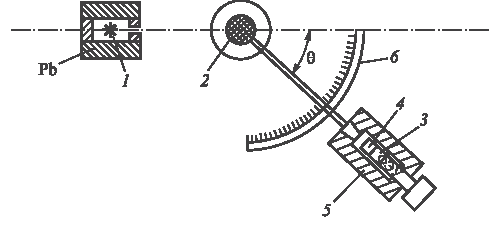
\includegraphics[scale=1]{ustanovka1.pdf}{\label{pic1}}}
				\ffigbox[\FBwidth]{\caption{}}%
				{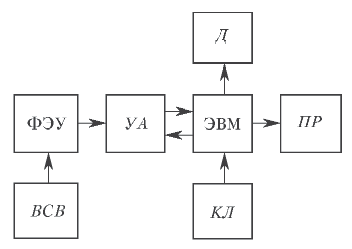
\includegraphics[scale=1]{ustanovka2.pdf}{\label{pic2}}}         
			\end{subfloatrow}
		}
		{\caption{Экспериментальная установка.}}
	\end{figure}
	
	Кванты, испытавшие комптоновское рассеяние в мишени, региструруются сцинтилляционным счетчиком. Счетчик состоит из фотоэлектронного умножителя 3 (далее ФЭУ) и сцинтиллятора 4. Сцинтиллятором служит кристалл NaI(Tl) цилиндрической формы диаметром 40 мм и высотой 40 мм, его выходное окно находится в оптическом контакте с фотокатодом ФЭУ. Сигналы, возникающие на ФЭУ, подаются на ЭВМ для амплитудного анализа. Кристалл и ФЭУ расположены в светонепроницаемом блоке, укрепленном на горизонтальной штанге. Штанга вместе с этим блоком может вращаться относительно мишени, угол поворота отсчитывается по лимбу 6.
	
	На рис.~\ref{pic2} представлена функциональная блок-схема измерительного комплекса, который состоит из ФЭУ, питаемого от высоковольтного выпрямителя ВСВ, обеспечивающего работу ФЭУ в спектрометрическом режиме, усилителя-анализатора УА, являющегося входным интерфейсом ЭВМ, управляемой с клавиатуры КЛ. В ходе проведения эксперимента информация отражается на экране дисплея Д, окончательные результаты в виде таблиц и графиков могут быть выведены на принтер ПР.
	
	\newpage
	\section{Экспериментальные данные}
	
		\floatsetup[table]{capposition=top}	
		\begin{table}[H]
			\caption{Измеряемые величины и их погрешность.}
			\label{table:parametr}
			\begin{tabular}{|c|c|c|c|}
				\hline
				$\theta$, $^\circ$ & $\sigma_\theta$, $^\circ$ & $N$ & $\sigma_N$ \\ \hline
				0,0                & \multirow{11}{*}{0,5}     & 790 & 20         \\ \cline{1-1} \cline{3-4} 
				10,0               &                           & 770 & 10         \\ \cline{1-1} \cline{3-4} 
				20,0               &                           & 680 & 30         \\ \cline{1-1} \cline{3-4} 
				30,0               &                           & 630 & 20         \\ \cline{1-1} \cline{3-4} 
				40,0               &                           & 590 & 40         \\ \cline{1-1} \cline{3-4} 
				50,0               &                           & 530 & 40         \\ \cline{1-1} \cline{3-4} 
				60,0               &                           & 440 & 50         \\ \cline{1-1} \cline{3-4} 
				70,0               &                           & 400 & 50         \\ \cline{1-1} \cline{3-4} 
				80,0               &                           & 350 & 40         \\ \cline{1-1} \cline{3-4} 
				90,0               &                           & 320 & 50         \\ \cline{1-1} \cline{3-4} 
				100,0              &                           & 300 & 50         \\ \hline
			\end{tabular}
		\end{table}
	
	
		\floatsetup[table]{capposition=top}	
		\begin{table}[H]
			\caption{Счетная характеристика ФЭУ № 4012.}
			\label{table:schet}
			\begin{tabular}{|c|c|c|c|c|}
				\hline
				$t$, с              & $U$, кВ & $\sigma_U$, кВ       & Счет  & $\sigma_\text{Счет}$   \\ \hline
				\multirow{7}{*}{60} & 1,2     & \multirow{7}{*}{0,5} & 16000 & \multirow{7}{*}{2000} \\ \cline{2-2} \cline{4-4}
				& 1,3     &                      & 51000 &                       \\ \cline{2-2} \cline{4-4}
				& 1,4     &                      & 63000 &                       \\ \cline{2-2} \cline{4-4}
				& 1,5     &                      & 63000 &                       \\ \cline{2-2} \cline{4-4}
				& 1,6     &                      & 71000 &                       \\ \cline{2-2} \cline{4-4}
				& 1,7     &                      & 69000 &                       \\ \cline{2-2} \cline{4-4}
				& 1,8     &                      & 71000 &                       \\ \hline
			\end{tabular}
		\end{table}
	

		
	\newpage
	\section{Обработка результатов}
		Оценим погрешности величин $1 - \cos \theta$ и $1/N$ по следующим формулам:
		\begin{equation*}
			\sigma_{1-\cos \theta} = \sin \theta \cdot \sigma_\theta, \ \sigma_{1/N} = 1/N^2 \cdot \sigma_N.
		\end{equation*}
			
		Результаты вычислений представлены в следующей таблице:
			
		\floatsetup[table]{capposition=top}	
		\begin{table}[H]
			\caption{Обработанные данные.}
			\label{table:data}
			\begin{tabular}{|c|c|c|c|}
				\hline
				$1 - \cos \theta$ & $\sigma_{1-\cos \theta}$ & $1/N \cdot 10^3$ & $\sigma_{1/N}$ \\ \hline
				0,000             & 0                        & 1,27  & 0,02           \\ \hline
				0,015             & 0,002                    & 1,30  & 0,02           \\ \hline
				0,060             & 0,003                    & 1,48  & 0,05           \\ \hline
				0,134             & 0,004                    & 1,58  & 0,04           \\ \hline
				0,234             & 0,006                    & 1,7   & 0,1            \\ \hline
				0,357             & 0,007                    & 1,9   & 0,1            \\ \hline
				0,500             & 0,008                    & 2,3   & 0,2            \\ \hline
				0,658             & 0,008                    & 2,5   & 0,3            \\ \hline
				0,826             & 0,009                    & 2,9   & 0,3            \\ \hline
				1,000             & 0,009                    & 3,1   & 0,4            \\ \hline
				1,174             & 0,009                    & 3,4   & 0,6            \\ \hline
			\end{tabular}
		\end{table}
		
		Изобразим экспериментальные результаты (табл.~\ref{table:data}) в виде графика (рис.~\ref{fig:graph}). Согласно формуле (\ref{kek}) экспериментальные точки должны лежать на одной прямой, что, как видно, выполняется. Пересечение этой прямой с осью ординат определяет наилучшее значение $N_\text{наил}(0)$, а пересечение линии $1 - \cos \theta = 1$ позволяет найти наилучшее значение $N_\text{наил}(90)$. 
	
	
		\begin{figure}[h!]
			\begin{floatrow}
				\ffigbox[\FBwidth]{\caption{Зависимость $1/N = f (1 - \cos \theta)$.}\label{fig:graph}}%
				{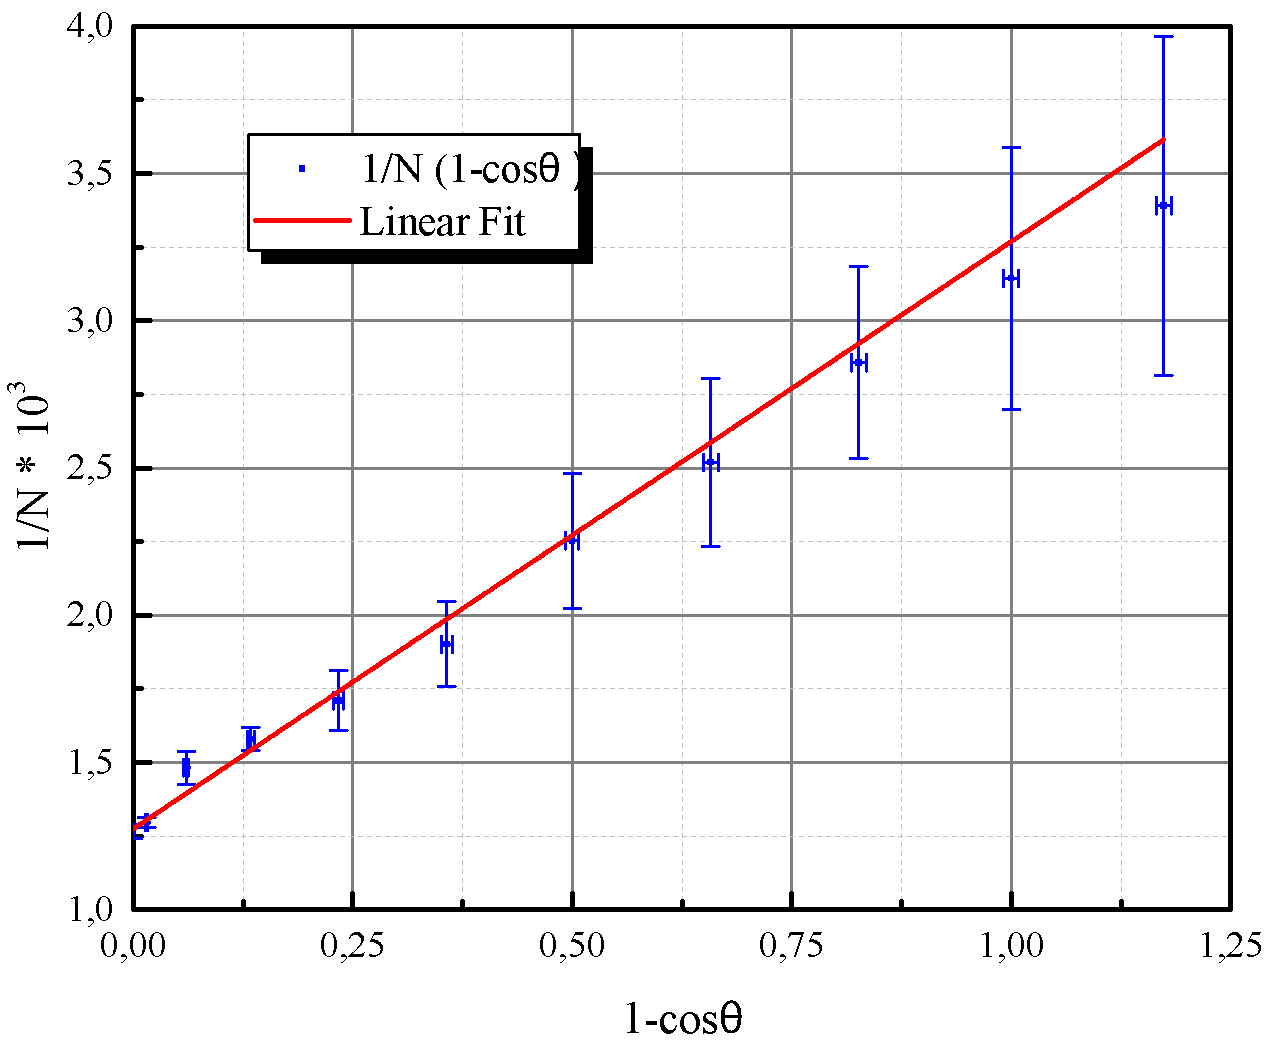
\includegraphics[scale=0.41]{graph1.pdf}}       
			\end{floatrow}
		\end{figure}

		\begin{table}[h!]
			\begin{floatrow}
				\ttabbox[\FBwidth]{\caption{$f(x) = Ax + B$.}\label{a,b}}%
				{\begin{tabular}{|c|c|c|}
						\hline
						$A \cdot 10^3$ & $B\cdot 10^3$   & $R^2$ \\ \hline
						$2,0 \pm 0,1$  & $1,27 \pm 0,01$ & 0,97  \\ \hline
			\end{tabular}}
				%\ttabbox[\FBwidth]{\caption{Наил. $N^{-1}$}\label{N-1}}%
				%{\begin{tabular}{|c|c|}
				%		\hline
				%		$N_\text{наил}^{-1}(0)$ & $N_\text{наил}^{-1}(90)$ \\ \hline
				%		$1,27 \pm 0,01$  & $3,3 \pm 0,1$   \\ \hline
				%\end{tabular}} 
				\ttabbox[\FBwidth]{\caption{Наил. $N$}\label{N}}%
				{\begin{tabular}{|c|c|}
						\hline
						$N_\text{наил}(0)$ & $N_\text{наил}(90)$ \\ \hline
						$769 \pm 6$  & $303 \pm 9$   \\ \hline
				\end{tabular}}       
			\end{floatrow}
		\end{table}
		
		\newpage
		Определим счетную характеристику $y(U)$ ФЭУ №4012 на основе результатов измерений, представленных в таблице~$\ref{table:schet}$. Это позволит нам учесть случайные ошибки, обсуловленные скачками напряжений, сильно влияющими на коэффциицент усиления ФЭУ.
		
		\begin{figure}[h!]
			\begin{floatrow}
				\ffigbox[\FBwidth]{\caption{Счетная характеристика ФЭУ № 4012.}\label{fig:U}}%
				{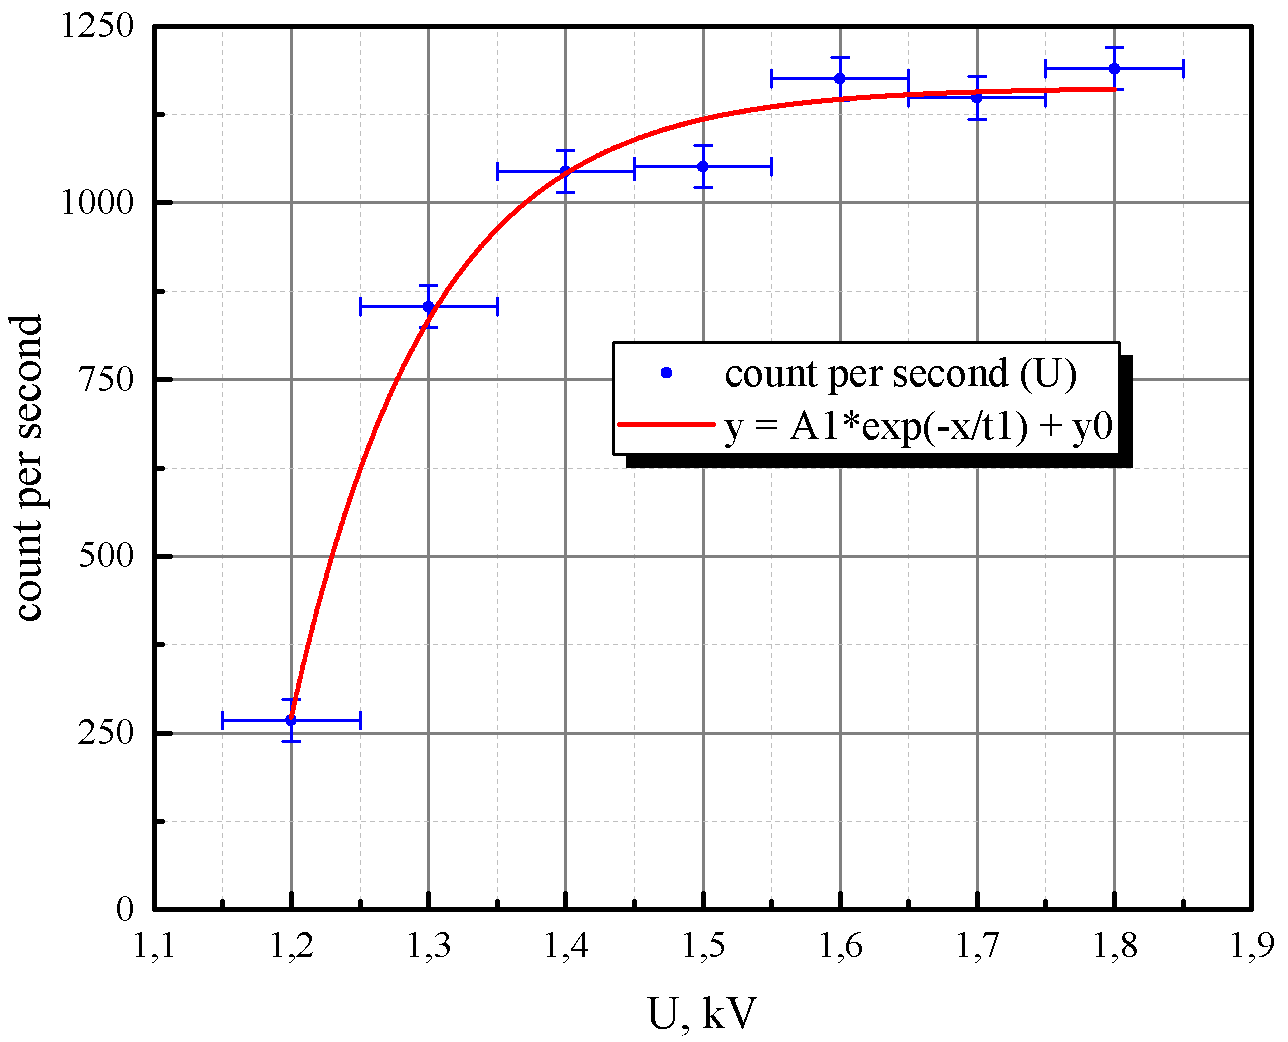
\includegraphics[scale=0.5]{graph2.pdf}}        
			\end{floatrow}
		\end{figure}
	
		Вид зависимости найдем в следующем виде:
		\begin{equation*}
			y (U) = A_1 e^{-U/t_1} + y_0.
		\end{equation*}
	
		\floatsetup[table]{capposition=top}	
		\begin{table}[H]
			\caption{Параметры аппроксимации $y(U)$.}
			\label{table:exp}
			\begin{tabular}{|c|c|c|c|}
				\hline
				$y_0$, cчет/c & $A_1$, счет/c$\cdot 10^8$ & $t_1$, кВ & $R^2$ \\ \hline
				$1160 \pm 20$ & $-1 \pm 2$                & $0,10 \pm 0,01$  & 0,98  \\ \hline
			\end{tabular}
		\end{table}
\newpage
\section{Обсуждение результатов и выводы}
	Итак, в настоящей лабораторной работе нами была проведена проверка соотношения (\ref{Kompton}). Экспериментально установлено, что $\gamma$-кванты действительно испытывают упругое рассеяние на свободных частицах. 
	
	Обратим наше внимание на то, что с увеличением угла $\theta$ погрешность измерения номера канала $\sigma_N$ увеличивается, что связано со смещением фотопика в сторону сплошного распределения, обязанного комптоновскому рассеянию. При $\theta = 110^\circ$ уже было невозможно увидеть пик полного поглощения.
	
	На основании таблицы \ref{N} можно определить энергию покоя частиц, на которых происходит комптоновское рассеивание. Путем несложных преобразований формула (\ref{1-cos}) принимает вид:
	\begin{equation*}
		mc^2 = E(0) \frac{N_\text{наил}(90)}{N_\text{наил}(0)-N_\text{наил}(90)},
	\end{equation*}
	где $E(0)$ -- энергия $\gamma$-лучей, испускаемых источником (в нашем случае $^{137}$Cs), то есть 662 кэВ. Имеем:
	\[
	\boxed{mc^2 = 430 \pm 20 \ \text{кэВ}}.
	\]
	Видно, что результат на 16\% меньше 511 кэВ -- энергии покоя электрона. Почему? Погрешность должна быть больше...
	
	Отметим, что колебания напряжения на ФЭУ № 4012 практически не вносят погрешности в измерения, ведь в работе было использовано напряжение $U = 1,6$ кэВ, при котором счетная характеристика выходит на константу, как видно из рисунка~\ref{fig:U}.
	
	
	
	
\end{document}